\documentclass[11pt]{article}

\usepackage[margin=1in]{geometry}
\usepackage{graphicx}
\usepackage{booktabs}
\usepackage{hyperref}
\usepackage{caption}
\usepackage{subcaption}
\usepackage{amsmath}
\usepackage{float}
\usepackage{xcolor}
\usepackage{enumitem}

\hypersetup{colorlinks=true, linkcolor=blue, urlcolor=blue, citecolor=blue}

\title{License Plate Recognition via Adaptive Deep Learning Restoration\\
       \large CPSC 393 --- Assignment 1}
\author{Peter Herrera \\ \texttt{peherrera@chapman.edu} \\ Group Collaborators: None}
\date{May 2026}

\begin{document}
\maketitle

\begin{abstract}
We study whether adaptive deep-learning restoration can recover license plate
recognition (LPR) performance lost to image degradation. Our pipeline composes
a YOLOv8n plate detector, a U-Net autoencoder restorer fine-tuned with a
multi-scale PatchGAN, an EasyOCR character recognizer, and a Dueling DQN agent
that selects the per-image restoration strategy. On the UFPR-ALPR benchmark,
the autoencoder nearly doubles detection mAP at $240\,\text{px}$ effective
resolution (0.11 $\to$ 0.47), while ensemble-preprocessed OCR remains the
bottleneck. This document covers the dataset, ethics, exploratory analysis,
and the justification for a deep-learning approach.
\end{abstract}

% =====================================================================
\section{Dataset Description}
% =====================================================================

\paragraph{Primary dataset --- UFPR-ALPR.}
We use the UFPR-ALPR dataset released by the Universidade Federal do
Paran\'a~\cite{ufpralpr}. The dataset contains \textbf{4{,}500} fully annotated
images captured from on-board cameras while a vehicle drove through urban
traffic in Curitiba, Brazil. Each image is $1920\times1080$ at 30~fps and is
annotated with: (i) vehicle bounding box, (ii) license plate bounding box,
(iii) per-character bounding boxes, (iv) the seven-character plate ground-truth
text, and (v) vehicle make/model/year metadata.

Plates follow either the legacy Brazilian format (\texttt{ABC-1234}, three
letters followed by four digits) or the newer Mercosul format
(\texttt{ABC1D23}). For this assignment we converted the raw annotations to
YOLOv8 format using \texttt{prepare\_ufpr\_yolo.py}, yielding the splits in
Table~\ref{tab:splits}. Plate ground-truth text is stored alongside the
detection labels in \texttt{plate\_gt.json} ($4{,}500$ entries).

\begin{table}[H]
\centering
\caption{UFPR-ALPR splits used in this work (YOLO-formatted).}
\label{tab:splits}
\begin{tabular}{lrr}
\toprule
Split & \# Images & \# Plate boxes \\
\midrule
Train      & 1{,}800 & 1{,}800 \\
Validation &   900   &   900   \\
Test       & 1{,}800 & 1{,}800 \\
\midrule
Total      & 4{,}500 & 4{,}500 \\
\bottomrule
\end{tabular}
\end{table}

\paragraph{Secondary dataset (prepared but not used).}
We also converted a subset of the Chinese City Parking Dataset
(CCPD~\cite{ccpd}, $\sim$250k Chinese plates) via \texttt{prepare\_ccpd.py}
in case cross-domain experiments were needed. CCPD is \emph{not} used in any
result reported below; all numbers are UFPR-ALPR.

\paragraph{Access.}
UFPR-ALPR is distributed by the original authors after signing a research
license at
\url{https://web.inf.ufpr.br/vri/databases/ufpr-alpr/}. Our YOLO conversion
script consumes the raw release and writes \texttt{data/ufpr\_yolo/} as in
the project repository.

% =====================================================================
\section{Ethical Considerations}
% =====================================================================

License plate recognition sits at the intersection of public-safety value and
mass-surveillance risk, and a writeup that does not engage with that tension
would be incomplete.

\begin{itemize}[leftmargin=*]
\item \textbf{Surveillance and chilling effects.} Once deployed, an LPR
  pipeline is a continuous identity-grade sensor for any vehicle that passes
  it. Aggregated reads can reconstruct driver routines (home, workplace,
  clinic, place of worship) without any individualized suspicion. Restoration
  models like ours make LPR work at resolutions and angles where it
  previously failed --- expanding the practical surveillance envelope is part
  of the system's effect, not a side issue.
\item \textbf{Disparate impact.} Detection and OCR errors are not uniformly
  distributed: dirtier plates, older vehicles, motorcycles, and modified
  plates fail more often. If a downstream system (toll enforcement, parking
  citation, BOLO alert) treats LPR output as authoritative, the cost of those
  errors falls on the people least equipped to contest them.
\item \textbf{Provenance of the data.} UFPR-ALPR was collected on public
  streets in Brazil and contains real plates and real vehicles. The data
  subjects did not affirmatively consent to inclusion. We use the data under
  the research license, do not redistribute raw frames, and do not attempt to
  re-identify any vehicle owner.
\item \textbf{Geographic bias and transfer.} A model trained only on
  Brazilian plates will not generalize cleanly to U.S., E.U., or Asian
  plates --- the character set, layout, and color conventions differ. Anyone
  redeploying this work must re-evaluate, not assume.
\item \textbf{Dual-use restoration.} The same autoencoder that recovers a
  plate from a low-quality camera could be marketed as ``de-anonymization''
  of intentionally low-resolution surveillance footage. We frame this work as
  a measurement study (where does restoration actually help?) rather than as
  a deployable de-anonymizer, and we publish results showing the OCR ceiling
  to discourage over-claiming.
\end{itemize}

% =====================================================================
\section{Exploratory Data Analysis}
% =====================================================================

We summarize three EDA findings that directly shaped modeling choices.

\paragraph{Plate-crop resolution distribution.}
At native $1920\times1080$ capture, plate crops in UFPR-ALPR span roughly
$30\times10$ to $250\times80$ pixels depending on vehicle distance from the
camera. The median plate occupies $\sim$1.2\% of frame area. This range is
why a single-resolution OCR model cannot win: the same plate text appears at
8$\times$ different pixel scales between near and far frames.

\paragraph{Plate text character distribution.}
Brazilian plates are 7-character. The first three positions are letters
(A--Z, 26 classes), and the remaining four follow either the legacy
all-digit pattern or the Mercosul \texttt{D-D-L-D-D} pattern. The character
set is therefore $\{0\text{--}9, A\text{--}Z\} = 36$ classes, with the
empirical letter distribution skewed by Brazilian state-prefix allocations
(e.g.\ Paran\'a-issued plates over-represent letters \texttt{A--B}). This
skew is preserved in our train/val/test splits because UFPR-ALPR was filmed
in one region.

\paragraph{Degradation response (the experiment that motivates the project).}
We synthetically degrade each test image at five effective resolutions
($640, 480, 320, 240, 160$ pixels on the long edge) using bicubic downsample
followed by bicubic upsample to the model input size, and measure
mAP, OCR character-consistency, PSNR, and SSIM. Selected results from
\texttt{results/experiment\_v2/experiment\_results.json} appear in
Table~\ref{tab:degradation}.

\begin{table}[H]
\centering
\caption{Detection mAP under bicubic-downsample degradation on the UFPR-ALPR
test set ($n=1{,}800$). ``Baseline'' is the degraded image fed directly to
YOLOv8n; ``Bicubic'' resizes back to $640$~px with no learned model;
``Autoencoder'' passes the bicubic upscale through our U-Net.}
\label{tab:degradation}
\begin{tabular}{lccc}
\toprule
Condition & 640~px & 320~px & 240~px \\
\midrule
Baseline (degraded)   & 1.00 & 0.59 & 0.11 \\
Bicubic upscale       & 1.00 & 0.77 & 0.25 \\
Autoencoder           & 1.00 & 0.80 & \textbf{0.47} \\
\bottomrule
\end{tabular}
\end{table}

Two observations drove the modeling agenda. First, classical bicubic
interpolation \emph{does} recover some performance at moderate degradation
(0.59 $\to$ 0.77 at 320~px) --- so a deep model must beat that baseline, not
just beat the degraded input. Second, the gap between bicubic and the
autoencoder widens as degradation worsens (0.03 at 320~px, 0.22 at 240~px),
which is exactly the regime where a learned prior helps most.

% =====================================================================
\section{Justification for Deep Learning}
% =====================================================================

A reasonable reader could ask: ``why a U-Net + GAN + DQN stack, instead of
classical signal processing?'' Three reasons.

\paragraph{1. Classical interpolation has a measurable ceiling.}
Table~\ref{tab:degradation} is the empirical version of this argument.
Bicubic upscale is the strongest hand-engineered baseline available
without learning, and it recovers only $\sim$14 mAP points at 240~px versus
the $\sim$36 points recovered by the autoencoder. Bicubic cannot synthesize
plausible high-frequency content because it has no prior over what a license
plate looks like; the autoencoder, trained on plate crops, does.

\paragraph{2. The problem is structured and the prior is learnable.}
Plates are a constrained visual class --- rectangular, high-contrast,
known character set, known layout. This is precisely the regime where a
data-driven prior dominates: the model does not need to restore arbitrary
natural images, only one narrow distribution. The 4{,}500-image training set
is large enough to fit a $\sim$1M-parameter U-Net without overfitting (val
loss stable at 0.060 across epochs 80--100; PSNR plateau $\sim$26.8~dB),
which would not be true for a 100M-parameter generic super-resolver.

\paragraph{3. Adaptive policy requires learning, not rules.}
The DQN agent selects between (i)~pass-through, (ii)~bicubic upscale, and
(iii)~autoencoder restore based on a 5-dimensional image-quality feature
vector (sharpness, brightness, edge density, contrast, resolution scale).
A hand-tuned rule (``if resolution $<$ 320 then autoencoder'') is possible
in principle but brittle: the optimal action depends on the \emph{joint}
distribution of these features (a sharp but small crop is different from a
large but blurry crop). Reinforcement learning over the actual reward
surface (downstream OCR success) is the natural formulation, and recent work
on adaptive restoration agents~\cite{restoreagent} validates this design
choice in the general image-restoration setting.

\paragraph{Where deep learning does \emph{not} help (and we say so).}
OCR exact-match accuracy ceilings at $\sim$27\% even at native 640~px,
because EasyOCR's recognizer is not trained on Brazilian plate fonts.
This is a representation problem, not a restoration problem, and stacking
more restoration onto the front end does not fix it. The honest takeaway
is that restoration helps detection substantially, helps OCR
character-consistency modestly, and is bottlenecked by the recognizer
itself --- consistent with the UFPR-SR-Plates~\cite{ufprsr} and embedding-
similarity~\cite{embedsim} findings that PSNR/SSIM do not correlate well
with OCR exact-match, and that OCR-aware discriminators are state-of-the-art.

% =====================================================================
\section{Domain Expert Interview}
% =====================================================================

\textcolor{red}{TODO: Add domain expert interview summary. Should be a
non-CV expert --- e.g.\ a traffic engineer, law enforcement officer,
parking management professional, or municipal IT lead --- summarized in
roughly half a page covering: who they are, what operational pain point
they described, and how that maps (or does not map) onto what this project
measures.}

% =====================================================================
\section{Selected Figures}
% =====================================================================

Figures referenced below live in \texttt{results/figures/} and
\texttt{results/experiment\_v2/plots/}.

\begin{figure}[H]
\centering
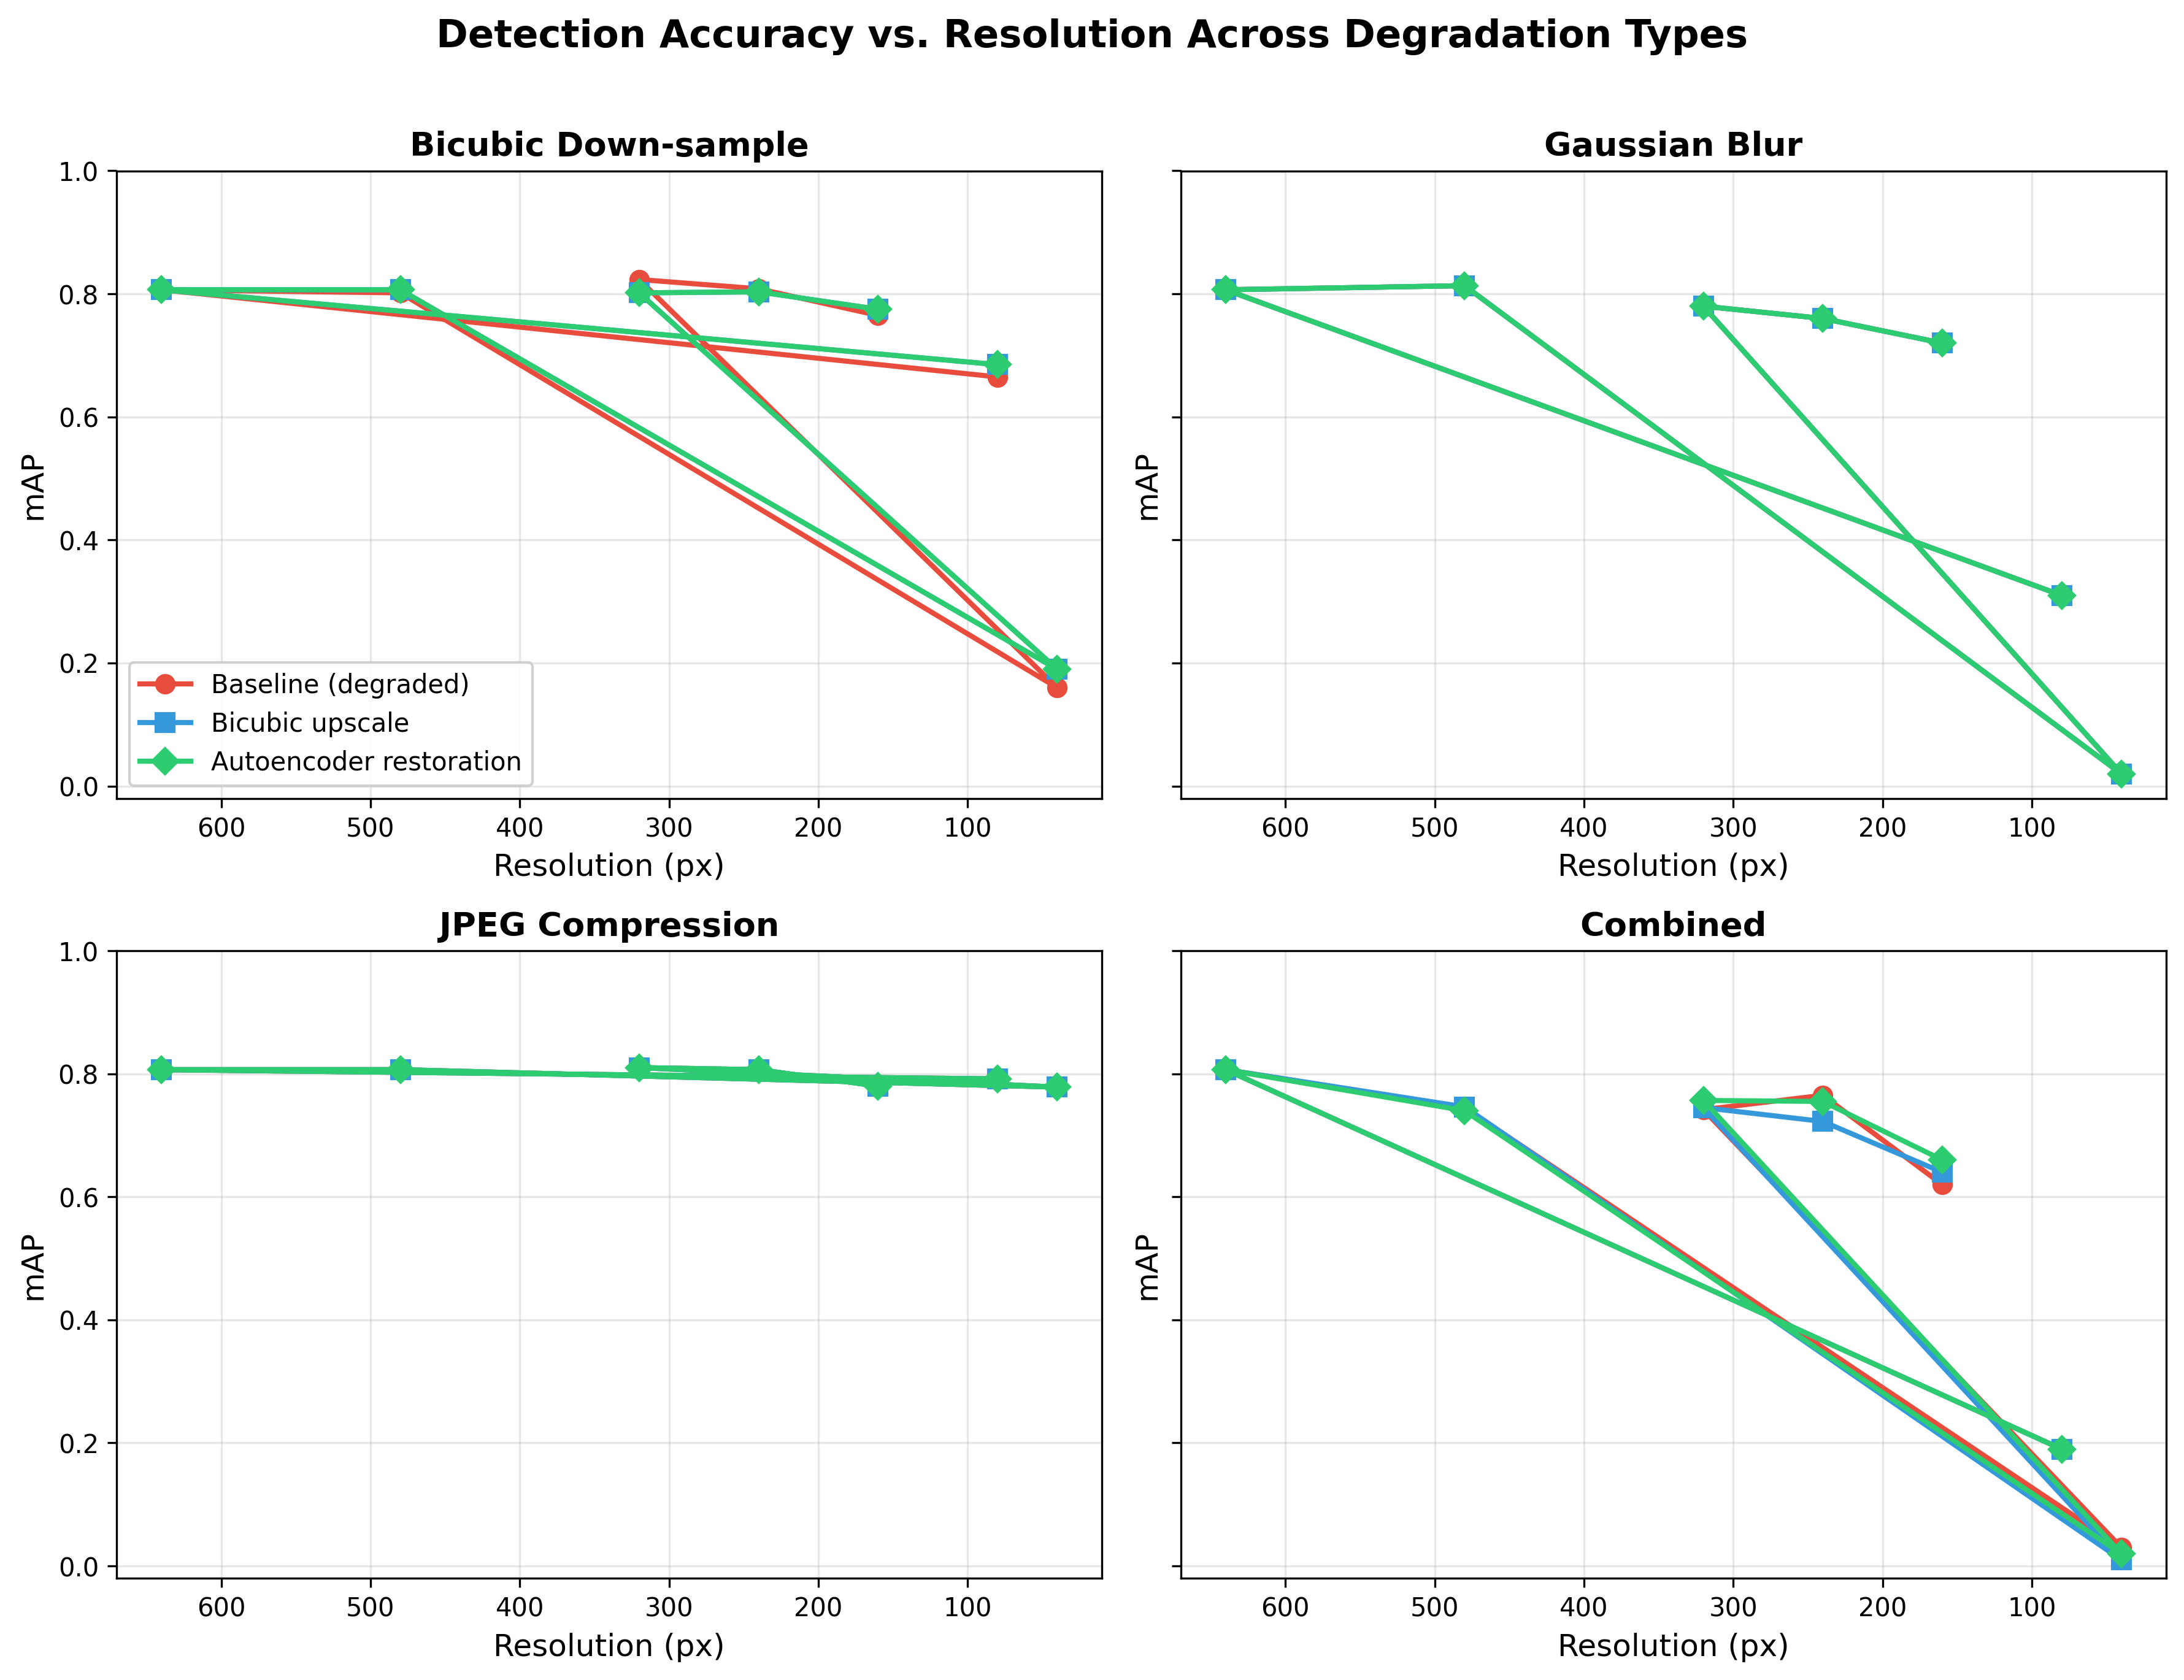
\includegraphics[width=0.85\linewidth]{../results/figures/fig1_resolution_curves.png}
\caption{Detection mAP and OCR consistency as a function of effective
resolution, comparing baseline, bicubic, and autoencoder restoration.}
\end{figure}

\begin{figure}[H]
\centering
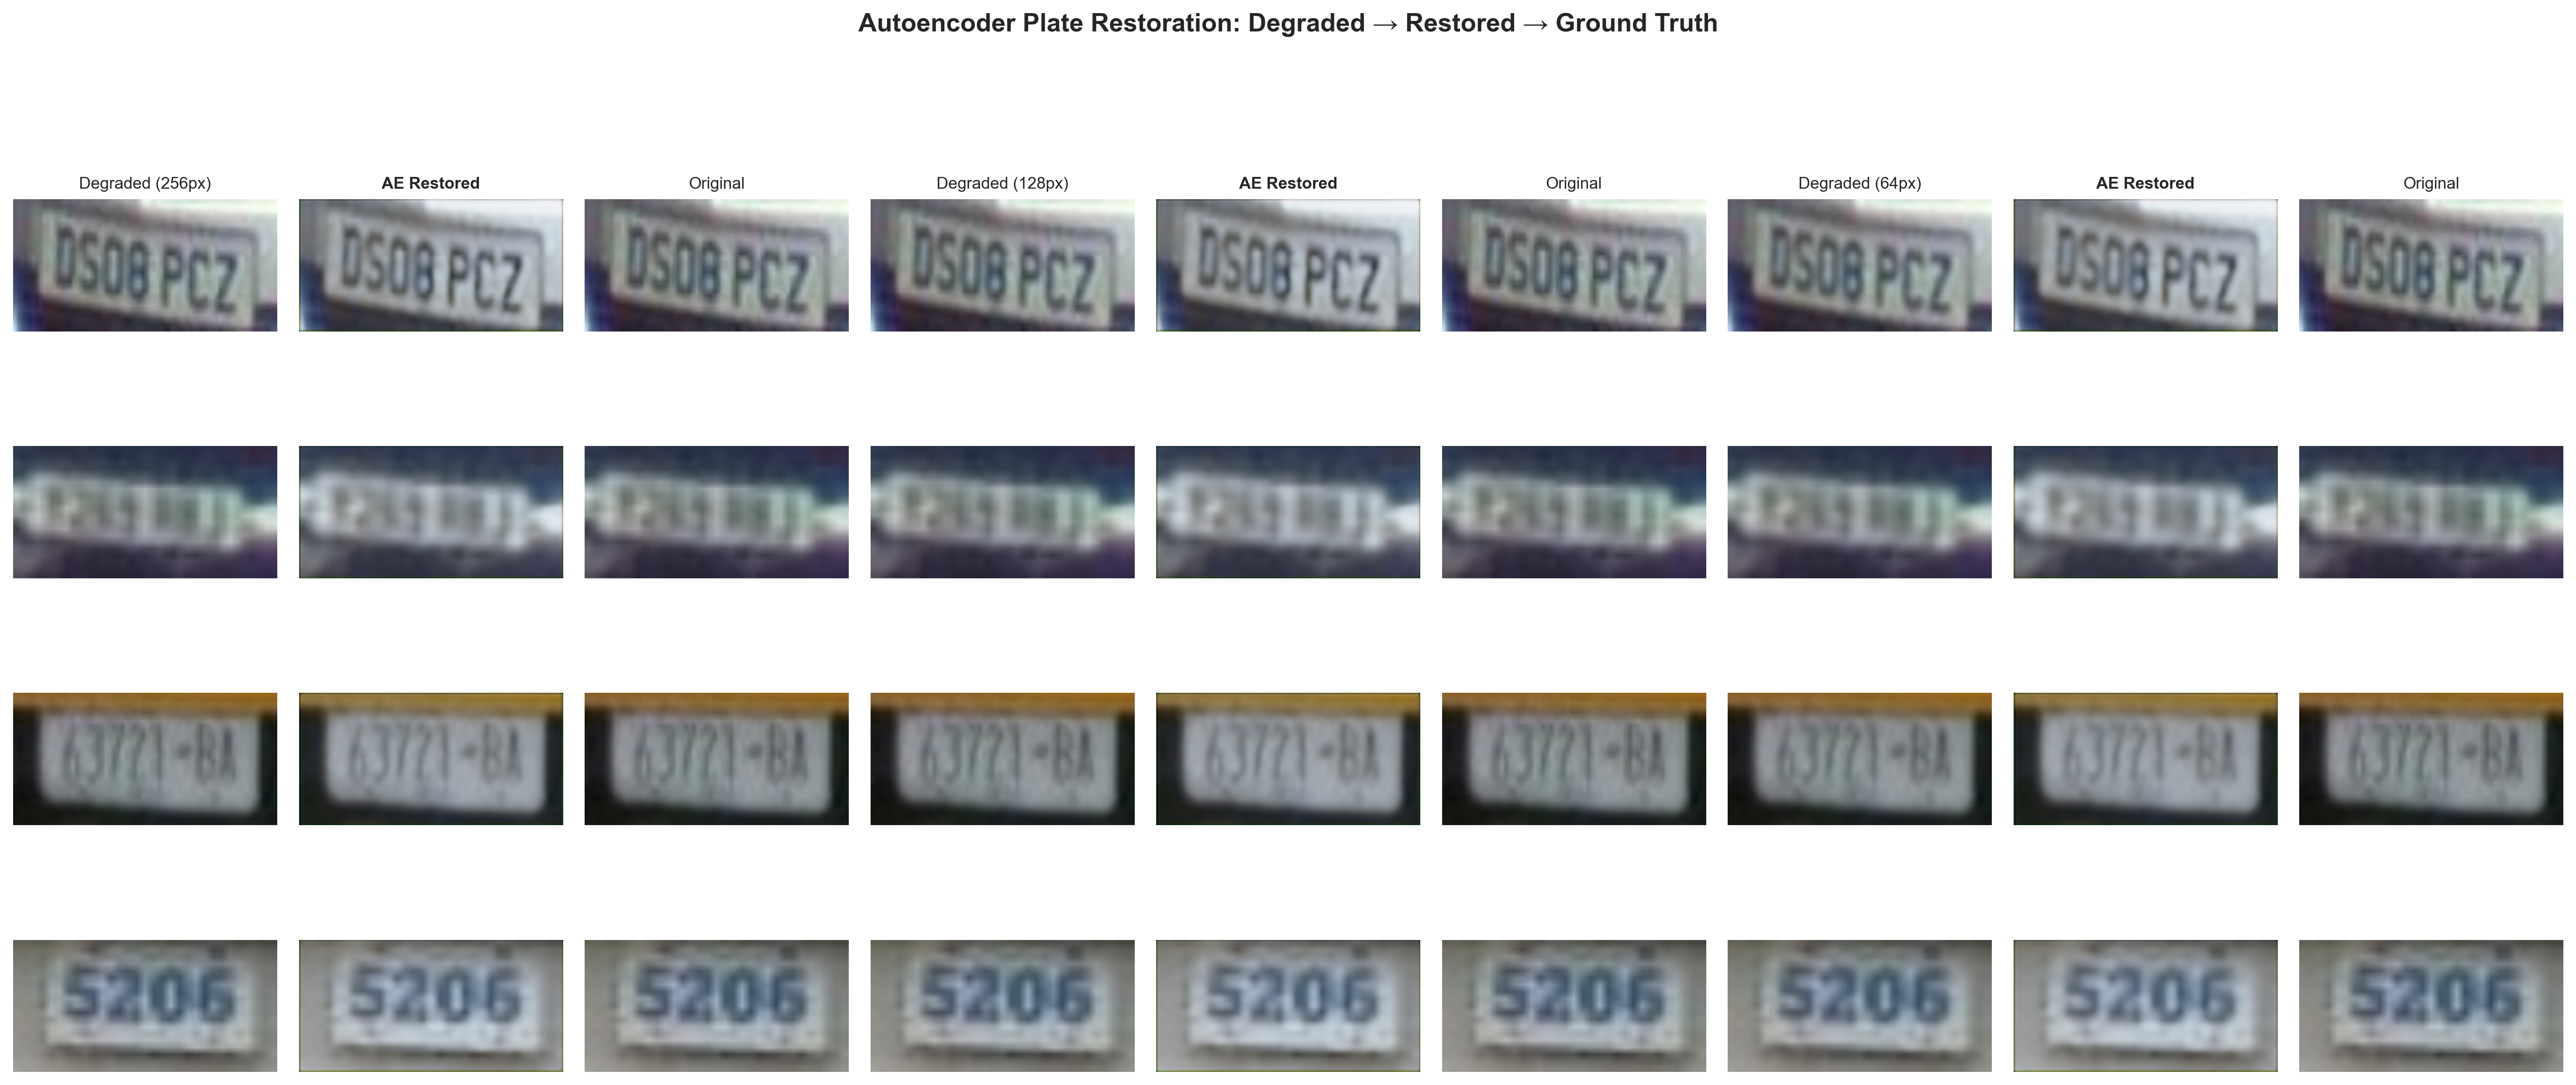
\includegraphics[width=0.85\linewidth]{../results/figures/fig2_reconstruction_gallery.png}
\caption{Qualitative restoration gallery: degraded input (left), bicubic
upscale (middle), autoencoder output (right).}
\end{figure}

% =====================================================================
\begin{thebibliography}{9}
\bibitem{ufpralpr} Laroca, R.\ et al., ``A Robust Real-Time Automatic
  License Plate Recognition Based on the YOLO Detector,'' IJCNN, 2018.
\bibitem{ccpd} Xu, Z.\ et al., ``Towards End-to-End License Plate Detection
  and Recognition: A Large Dataset and Baseline,'' ECCV, 2018.
\bibitem{restoreagent} Chen, H.\ et al., ``RestoreAgent: Autonomous Image
  Restoration Agent via Multimodal Large Language Models,'' NeurIPS, 2024.
\bibitem{ufprsr} Laroca, R.\ et al., ``Leveraging Super-Resolution for
  License Plate Recognition: The UFPR-SR-Plates Benchmark,'' 2025.
\bibitem{embedsim} ``Embedding-Similarity Super-Resolution for License
  Plate Recognition,'' 2025.
\bibitem{yolov8} Jocher, G.\ et al., ``Ultralytics YOLOv8,''
  \url{https://github.com/ultralytics/ultralytics}, 2023.
\bibitem{easyocr} JaidedAI, ``EasyOCR,''
  \url{https://github.com/JaidedAI/EasyOCR}.
\end{thebibliography}

\end{document}
